\documentclass[crop,tikz]{standalone}                 
\usepackage{physics}

\makeatletter                                                                                        

\newcommand{\sq}[1]{\frac{1}{\sqrt{#1}}}

\begin{document}

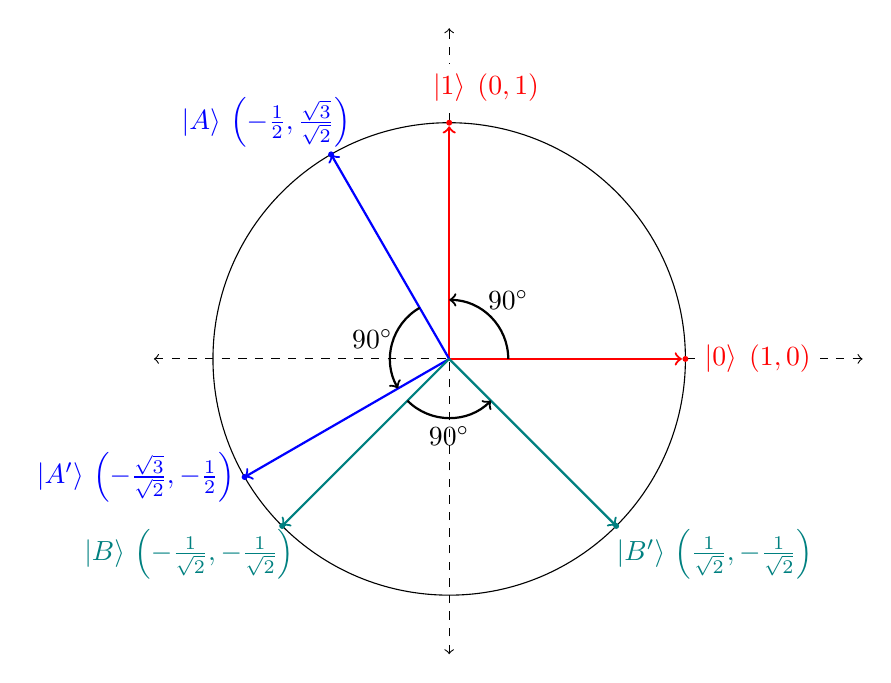
\begin{tikzpicture}[scale=1.5]                                                                          
\usetikzlibrary{positioning}
%\draw [dashed,gray, step=2cm] (-2.30,-2.30) grid ( 2.30, 2.30);

% Axes
%\draw [-] (-2.77164,-1.14805) -- (2.77164,1.14805);
\draw [<->, dashed] (0,-2.5) -- (0,2.8);
\draw [<->, dashed] (-2.5, 0) -- (3.5,0);

% Circle
\draw[] (0cm,0cm) circle(2.00cm);                                                                 

% Point ket-1
\filldraw[red] (0.00,2.00) circle (0.02cm);
\draw [->,thick,red] (0,0) -- (0.00, 1.97);
\node [fill=white,text=red] (ket1) at ( 0.00, 2.30) {$\ket{1}$};
\node [red]             (al) at ( 0.50, 2.30) {$(0,1)$};

% Point ket-0
\filldraw[red] ( 2.00, 0.00) circle (0.02cm);
\draw [->,thick,red] (0,0) -- (1.97, 0.00);
\node [fill=white, text=red] (ket2) at ( 2.30, 0.00) {$\ket{0}$};
\node [fill=white, text=red]   (al) at ( 2.80, 0.00) {$(1,0)$};

% Point ket-A
\filldraw[blue] (-1.00, 1.73205) circle (0.02cm);
\draw [->,thick,blue] (0,0) -- (-1.00, 1.73205);
\node [text=blue] (ket4) at (-1.55, 2.00205) {$\ket{A}$ $\left(-\frac{1}{2}, \frac{\sqrt{3}}{\sqrt{2}}\right)$};

% Point ket-A-prime
\filldraw[blue] (-1.73205, -1.00) circle (0.02cm);
\draw [->,thick,blue] (0,0) -- (-1.73205, -1.00);
\node [text=blue] (ket5) at (-2.65205, -1.00) {$\ket{A'}$ $\left(-\frac{\sqrt{3}}{\sqrt{2}},-\frac{1}{2}\right)$};

% Point ket-B
\filldraw[teal] (-1.41421, -1.41421) circle (0.02cm);
\draw [->,thick,teal] (0,0) -- (-1.41421, -1.41421);
\node [text=teal] (ket5) at (-2.20, -1.65) {$\ket{B}$ $\left(-\frac{1}{\sqrt{2}}, -\frac{1}{\sqrt{2}}\right)$};

% Point ket-B-prime
\filldraw[teal] (1.41421, -1.41421) circle (0.02cm);
\draw [->,thick,teal] (0,0) -- (1.41421, -1.41421);
\node [text=teal] (ket5) at ( 2.25, -1.65) {$\ket{B'}$ $\left(\frac{1}{\sqrt{2}}, -\frac{1}{\sqrt{2}}\right)$};

% Rotation Angles
\draw [->, thick] (  0 : 0.5) arc (  0 : 90  : 0.5);
\draw [->, thick] (120 : 0.5) arc (120 : 210 : 0.5);
\draw [->, thick] (225 : 0.5) arc (225 : 315 : 0.5);

% Angle Labels
\node [] (l1) at (0.5,0.5) {$90^\circ$};
\node [] (l1) at (-0.65, 0.17) {$90^\circ$};
\node [] (l1) at ( 0.0, -0.65) {$90^\circ$};

\end{tikzpicture}                                                                                    

\end{document}
